\documentclass{book}

\usepackage{amssymb}
\usepackage{amsmath}
\usepackage{amsthm}
\usepackage{arydshln}
\usepackage{calc}
\usepackage{cancel}
\usepackage{caption}
\usepackage{cite}
\usepackage{color}
\usepackage{enumitem}
\usepackage{esint}
\usepackage{etoolbox}
\usepackage{float}
\usepackage{framed}
\usepackage{fullpage}
\usepackage{gensymb}
\usepackage[margin=1in]{geometry}
\usepackage{graphicx}
\usepackage{listings}
\usepackage{multirow}
\usepackage{subfiles}
\usepackage{rsfso}
\usepackage{tikz}
\usepackage{tikz-3dplot}
\usepackage{ushort}
\usepackage{wrapfig}
\usepackage{xcolor}
\usepackage{soul}
\usepackage{epstopdf}

% pdf versions
\pdfoptionpdfminorversion=7

% handle page stretching
\raggedbottom

% Graphics file location
\graphicspath{{Graphics/}{../Graphics/}}

% Use for drawings
\usetikzlibrary{angles,arrows,calc,decorations,intersections,patterns,positioning,quotes,shapes}
\usetikzlibrary{shapes.geometric}
\usetikzlibrary{decorations.pathreplacing}
\newcommand{\midarrow}{\tikz \draw[-latex] (0,0) -- +(.1,0);}

% Tikz commands for drawing block diagrams, etc...
\tikzset{%
	block/.style    = {draw, rectangle, minimum height = 2em, minimum width = 2em},
	sum/.style      = {draw, circle}, % Adder
	input/.style    = {fill=white, rectangle}, % Input
	output/.style   = {fill=white, rectangle}, % Output
	waypoint/.style   = {coordinate}, % Output
}

\tikzset{%
	startstop/.style= {draw, rectangle, rounded corners, minimum width=2cm, minimum height=1cm,text centered},
	inout/.style    = {draw, trapezium, trapezium left angle=70, trapezium right angle=110, minimum width=2cm, minimum height=1cm, text centered},
	process/.style  = {draw, rectangle, minimum width=2cm, minimum height=1cm, text centered},
	decision/.style = {draw, diamond, minimum width=1.5cm, minimum height=1cm, text centered, diamond, aspect=2},
	arrow/.style    = {thick,-latex,>=stealth},		
}

\tikzset{
	saveuse path/.code 2 args={
		\pgfkeysalso{#1/.style={insert path={#2}}}%
		\global\expandafter\let\csname pgfk@\pgfkeyscurrentpath/.@cmd\expandafter\endcsname
		% not optimal as it is now global through out the document
		\csname pgfk@\pgfkeyscurrentpath/.@cmd\endcsname
		\pgfkeysalso{#1}},
	/pgf/math set seed/.code=\pgfmathsetseed{#1}}

% Define Laplace, Fourier transform symbols
\newcommand{\LT}{\mathcal{L}}
\newcommand{\FT}{\mathcal{F}}

% Define adjugate function
\newcommand{\adj}{\text{adj}}

% Define rank function
\newcommand{\rank}{\text{rank}}

% commands to speed up writing j\omega and s-plane
\newcommand{\jw}{j\omega}
\newcommand{\jt}{j\theta}
\newcommand{\wt}{\omega t}
\newcommand{\spl}{s\textrm{-plane}}
\newcommand{\Lm}{\textrm{Lm }}
% Clean up overline/underline for math mode
\def\obar#1{\bar{#1}}
\def\ubar#1{\ushort{#1}}

\newcommand{\exmp}{\subsubsection*{Example}}
\newcommand{\nib}{\noindent$ \bullet\ $}


\begin{document}
\chapter*{Lecture 4}
Last time:
\begin{itemize}
	\item Transfer Functions
	\item State-space forms
\end{itemize}

By this point, one should be familiar with the relationship between system representation in the complex plane (or $ s $-plane poles and zeros) and it's representation in the time domain (time plots).
Time domain:
\begin{center}	
	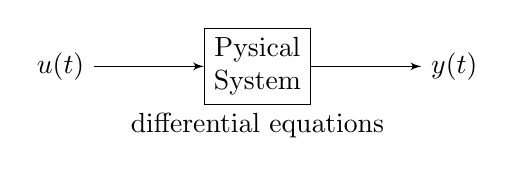
\begin{tikzpicture}[node distance=2.5cm,auto,>=latex']
	\node [input, align=center] (U) {$ u(t) $};
	\node [block, align=center] (G) [right of=U] {Pysical\\System};
	\node[below of=G,node distance=0.75cm] {differential equations};
	\node [output, align=center] (y) [right of=G] {$ y(t) $};
	\draw[->] (U) -- node {} (G);
	\draw[->] (G) -- node {} (y);
	\end{tikzpicture}
\end{center}
Laplace domain:
\begin{center}	
	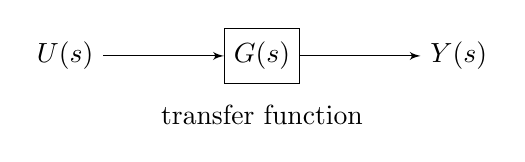
\begin{tikzpicture}[node distance=2.5cm,auto,>=latex']
	\node [input, align=center] (U) {$ U(s) $};
	\node [block, align=center] (G) [right of=U] {$ G(s) $};
	\node[below of=G,node distance=0.75cm] {transfer function};
	\node [output, align=center] (y) [right of=G] {$ Y(s) $};
	\draw[->] (U) -- node {} (G);
	\draw[->] (G) -- node {} (y);
	\end{tikzpicture}
\end{center}
In general, we have
\[ Y(s) = G(s)U(s) \]
where $ G(s) $ is proper or strictly proper (never improper) and $ U(s) $ is generally strictly proper. As a whole this means that $ Y(s) $ is generally strictly proper but at ``most'' it is proper.

As an example, consider the case for strictly proper with distinct poles for $Y(s) $.
\[ Y(s) = \frac{R_1}{s+p_1}+\frac{R_2}{s+p_2}+\ldots+\frac{R_n}{s+p_n} \]
\[ y(t) = \sum_{j=1}^{n} \LT^{-1} \left(\frac{R_j}{s+p_j}\right) = \sum_{j=1}^{n} R_j e^{-p_jt} \]
This is simply the sum of exponentials. Some of these may be complex, resulting in sines and cosines in the response. In general, the $ y(t) $ above will be the sum of simple time functions.
\begin{enumerate}
	\item If $ Y(s) $ has a pole at the origin of the complex plane, $ y(t) $ has a step function in the time domain.
	\item If $ Y(s) $ has a pole on the real axis, $ y(t) $ has an exponential function in the time domain.
	\begin{enumerate}
		\item negative real axis: decaying exponential
		\item positive real axis: growing exponential
	\end{enumerate}
	\item If $ Y(s) $ has a pair of poles on the imaginary axis, symmetrically placed with regards to the real axis (complex conjugates), then $ y(t) $ has undamped oscillations of frequency $ \omega $ (where $ \omega $ is the imaginary part of the poles). Explanation:
	\[ Y(s) = \frac{\omega}{s^2+\omega^2}  \quad\Rightarrow\quad \text{poles are given by }s^2+\omega^2=0 \Rightarrow s^2=-\omega^2 \Rightarrow s=\pm\jw \]
	But, for this $ Y(s) $, we know that $ y(t)=\sin\wt$ (undamped oscillation)
	\item If $ Y(s) $ has a pair of conjugate poles not on the imaginary axis, $ y(t) $ will have decaying or growing oscillations. Explanation:
	\[ \text{Decaying Oscillation ($ a>0 $): } y(t) = e^{-at}\sin\wt 1(t) \]
	\[ Y(s) = \LT[y(t)] = ? \]
	\[ \LT[\sin\wt 1(t)] = \frac{\omega}{s^2+\omega^2} \]
	\[ \LT[e^{-at}\sin\wt 1(t)] = \frac{\omega}{(s+a)^2+\omega^2} = Y(s) \]
	The poles of $ Y(s) $ are $ (s+a)^2+\omega^2=0 $. So,
	\[ (s+a)^2 = -\omega^2 \]
	\[ s+a = \pm \omega \]
	\[ s= -a\pm\jw \]
	Complex conjugate poles in left-hand plane
	\[ \text{Growing Oscillation ($ a>0 $): } y(t) = e^{+at}\sin\wt 1(t) \]
	Following the same steps,
	\[ Y(s) = \frac{\omega}{(s-a)^2+\omega^2} \]
	\[ s= a\pm\jw \]
	\item If $ Y(s) $ has multiple poles at the same location on complex plane, the time-domain counterpart of a single pole is multiplied by $ t $. For example, recall
	\[ \LT[tf(t)] = -\frac{d}{ds}F(s) \]
	So,
	\[ \LT[t\cdot e^{-at}1(t)] = -\frac{d}{ds}\frac{1}{s+a}=\frac{1}{(s+a)^2} \]
	\[ \LT[t\cdot \sin\wt 1(t)] = -\frac{d}{ds}\frac{\omega}{s^2+\omega^2}=\frac{2\omega s}{(s^2+\omega^2)^2} \]
	and of course
	\[ \LT[t1(t)] = -\frac{d}{ds}\frac{1}{s}=\frac{1}{s^2} \]
\end{enumerate}

Previously we looked at correspondences between the complex plane and the time domain.
\begin{center}
	\begin{tabular}{c c c c}
		Function $ f(t) $ & Plot of $ f(t) $ & $ F(s) $ & Pole-Zero Diagram \\ \hline\vspace{0.5em}
		$ 1(t) $ & 	\begin{tikzpicture}[scale=1]
		\draw[->] (-0.5,0) -- (2,0);  % x Axis
		\draw[->] (0,-0.25) -- (0,1.0);  % y Axis
		\node[below] at (1.9,0) {$ t $};
		\node[left] at (0,0.9) {$ f(t) $};
		\draw[domain=0:2] plot (\x,{.75});
		\end{tikzpicture}
		& $ \dfrac{1}{s} $ & \begin{tikzpicture}[scale=0.5]
		\draw (-2.5,0) -- (2.5,0) node[below left] {$ \sigma $};
		\draw (0,-1.5) -- (0,1.5) node[below left] {$ j\omega $};
		\node at (0,0) {\Large$ \times $};
		\end{tikzpicture} \\ \hline\vspace{0.5em}
		
		$ t1(t) $ & 	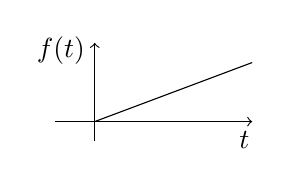
\begin{tikzpicture}
		\draw[->] (-0.5,0) -- (2,0);  % x Axis
		\draw[->] (0,-0.25) -- (0,1.0);  % y Axis
		\node[below] at (1.9,0) {$ t $};
		\node[left] at (0,0.9) {$ f(t) $};
		\draw[domain=0:2] plot (\x,{.375*\x});
		\end{tikzpicture} & $ \dfrac{1}{s^2} $ & 	\begin{tikzpicture}[scale=0.5]
		\draw (-3,0) -- (2,0) node[below left] {$ \sigma $};
		\draw (0,-1.5) -- (0,1.5) node[below left] {$ j\omega $};
		\node at (0,0) {\Large$ \times $};
		\node[above right] at (0,0) {$ 2 $};
		\end{tikzpicture} \\ \hline\vspace{0.5em}
		
		$ e^{-at}1(t) $ & 	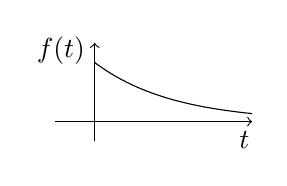
\begin{tikzpicture}
		\draw[->] (-0.5,0) -- (2,0);  % x Axis
		\draw[->] (0,-0.25) -- (0,1.0);  % y Axis
		\node[below] at (1.9,0) {$ t $};
		\node[left] at (0,0.9) {$ f(t) $};
		\draw[domain=0:2] plot (\x,{.75*exp(-\x)});
		\end{tikzpicture} & $ \dfrac{1}{s+a} $ & 	\begin{tikzpicture}[scale=0.5]
		\draw (-3,0) -- (2,0) node[below left] {$ \sigma $};
		\draw (0,-1.5) -- (0,1.5) node[below left] {$ j\omega $};
		\node at (-1,0) {\Large$ \times $};
		\node[below] at (-1,0) {$ a $};
		\end{tikzpicture} \\ \hline\vspace{0.5em}
		
		$ e^{at}1(t) $ & 	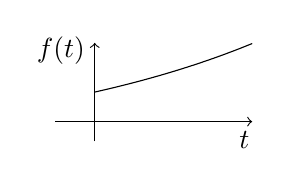
\begin{tikzpicture}
		\draw[->] (-0.5,0) -- (2,0);  % x Axis
		\draw[->] (0,-0.25) -- (0,1.0);  % y Axis
		\node[below] at (1.9,0) {$ t $};
		\node[left] at (0,0.9) {$ f(t) $};
		\draw[domain=0:2] plot (\x,{.75*exp(0.3*\x)-0.375});
		\end{tikzpicture} & $ \dfrac{1}{s+a} $ & 	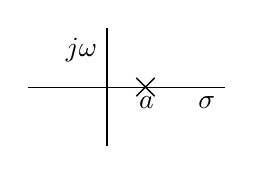
\begin{tikzpicture}[scale=0.5]
		\draw (-2,0) -- (3,0) node[below left] {$ \sigma $};
		\draw (0,-1.5) -- (0,1.5) node[below left] {$ j\omega $};
		\node at (1,0) {\Large$ \times $};
		\node[below] at (1,0) {$ a $};
		\end{tikzpicture} \\ \hline\vspace{0.5em}
		
		$ \cos\wt1(t) $ & 	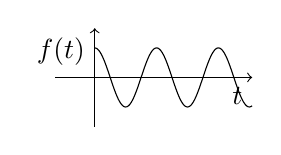
\begin{tikzpicture}[scale=1]
		\draw[->] (-0.5,0) -- (2,0);  % x Axis
		\draw[->] (0,-0.625) -- (0,0.625);  % y Axis
		\node[below left ] at (2,0) {$ t $};
		\node[below left] at (0,0.625) {$ f(t) $};
		\draw[domain=0:2,samples=240] plot (\x,{.375*cos((180/pi)*8*\x)});
		\end{tikzpicture} & $ \dfrac{s}{s^2+\omega^2} $ & 	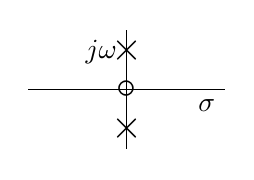
\begin{tikzpicture}[scale=0.5]
		\draw (-2.5,0) -- (2.5,0) node[below left] {$ \sigma $};
		\draw (0,-1.5) -- (0,1.5) node[below left] {$ j\omega $};
		\node at (0,1) {\Large$ \times $};
		\node at (0,-1) {\Large$ \times $};
		\node at (0,0) {\Large$ \circ $};
		\end{tikzpicture} \\ \hline\vspace{0.5em}
		
		$ \sin\wt1(t) $ & 	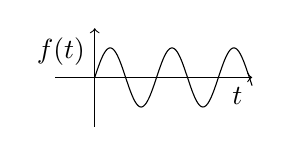
\begin{tikzpicture}
		\draw[->] (-0.5,0) -- (2,0);  % x Axis
		\draw[->] (0,-0.625) -- (0,0.625);  % y Axis
		\node[below left] at (2,0) {$ t $};
		\node[below left] at (0,0.625) {$ f(t) $};
		\draw[domain=0:2,samples=240] plot (\x,{.375*sin((180/pi)*8*\x)});
		\end{tikzpicture} & $ \dfrac{\omega}{s^2+\omega^2} $ & 	\begin{tikzpicture}[scale=0.5]
		\draw (-2.5,0) -- (2.5,0) node[below left] {$ \sigma $};
		\draw (0,-1.5) -- (0,1.5) node[below left] {$ j\omega $};
		\node at (0,1) {\Large$ \times $};
		\node at (0,-1) {\Large$ \times $};		
		\end{tikzpicture} \\  \hline\vspace{0.5em}	
		
		$ e^{-at}\sin\wt1(t) $ & 	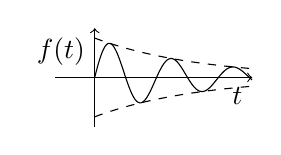
\begin{tikzpicture}
		\draw[->] (-0.5,0) -- (2,0);  % x Axis
		\draw[->] (0,-0.625) -- (0,0.625);  % y Axis
		\node[below left] at (2,0) {$ t $};
		\node[below left] at (0,0.625) {$ f(t) $};
		\draw[domain=0:2,samples=240] plot (\x,{.5*sin((180/pi)*8*\x)*exp(-0.75*\x)});
		\draw[dashed,domain=0:2,samples=240] plot (\x,{.5*exp(-0.75*\x)});
		\draw[dashed,domain=0:2,samples=240] plot (\x,{-.5*exp(-0.75*\x)});
		\end{tikzpicture} & $ \dfrac{\omega}{(s+a)^2+\omega^2} $ & 	\begin{tikzpicture}[scale=0.5]
		\draw (-2.5,0) -- (2.5,0) node[below left] {$ \sigma $};
		\draw (0,-1.5) -- (0,1.5) node[below left] {$ j\omega $};
		\node at (-1.25,1) {\Large$ \times $};
		\node at (-1.25,-1) {\Large$ \times $};		
		\end{tikzpicture} \\  \hline\vspace{0.5em}	
		
		$ e^{at}\sin\wt1(t) $ & 	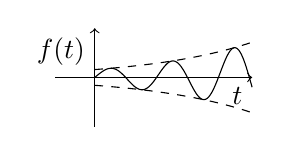
\begin{tikzpicture}
		\draw[->] (-0.5,0) -- (2,0);  % x Axis
		\draw[->] (0,-0.625) -- (0,0.625);  % y Axis
		\node[below left] at (2,0) {$ t $};
		\node[below left] at (0,0.625) {$ f(t) $};
		\draw[domain=0:2,samples=240] plot (\x,{.1*sin((180/pi)*8*\x)*exp(0.75*\x)});
		\draw[dashed,domain=0:2,samples=240] plot (\x,{.1*exp(0.75*\x)});
		\draw[dashed,domain=0:2,samples=240] plot (\x,{-.1*exp(0.75*\x)});
		\end{tikzpicture} & $ \dfrac{\omega}{(s-a)^2+\omega^2} $ & 	\begin{tikzpicture}[scale=0.5]
		\draw (-2.5,0) -- (2.5,0) node[below left] {$ \sigma $};
		\draw (0,-1.5) -- (0,1.5) node[below left] {$ j\omega $};
		\node at (1,1) {\Large$ \times $};
		\node at (1,-1) {\Large$ \times $};		
		\end{tikzpicture} \\	
	\end{tabular}
\end{center}
\begin{itemize}
	\item Poles in the LHP cause the time-domain equivalent to eventually decay to zero.
	\item Poles in the RHP cause the time domain equivalent to grow without bound. 
	\item For distinct poles on the $ \jw $ axis, the time domain signal is bounded but does not decay.
	\begin{itemize}
		\item Simple/single pole. This can only be at the origin and results in a step function in the time-domain.
		\item Complex conjugate poles. This results in undamped oscillations. 
		\item Multiple poles at the same location on the $ \jw $-axis have the time function multiplied by $ t $ (e.g. $ 1(t) \to t1(t) $), causing them to grow without bound. 
	\end{itemize}
\end{itemize}
\clearpage
Some observations:
\begin{itemize}
	\item The character of $ y(t) $ principally depends on the poles of $ Y(s) $ not on the zeros. For example:
	\[ Y(s) = \frac{\cdots}{s(s+a)(s^2+c^2)} \]
	Then $ y(t) $ consists of step, exponential, and sine/cosine responses. The zeros help determine the residuals, in other words the ``amount'' that each pole contributes to the total response.
	\item The equation that gives the poles of $ G(s) $ is often referred to as the characteristic equation.
	\[ \det(s\ubar{I}-\ubar{A})=0 \]
\end{itemize}

\subsection*{More on system response: Final Values, initial values, and static gain}
For a system $ S $, some given input $ u(t) $ gives rise to an output $ y(t) $.
\begin{center}
	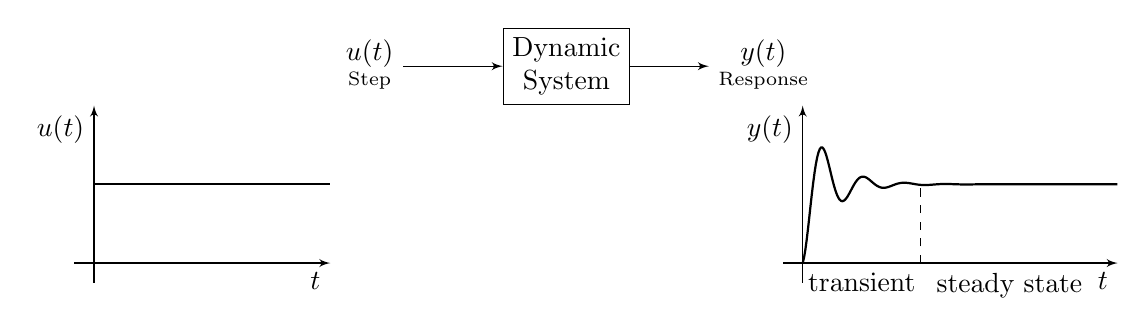
\begin{tikzpicture}[node distance=2.5cm,auto,>=latex']
	\node [input, align=center] (U) {$\underset{\text{Step}}{u(t)}$};
	\node [block, align=center] (G) [right of=U] {Dynamic\\System};
	\node [output, align=center] (y) [right of=G] {$\underset{\text{Response}}{y(t)}$};
	\draw[->] (U) -- node {} (G);
	\draw[->] (G) -- node {} (y);
	
	\begin{scope}[shift={(-3.5cm,-2.5cm)}]
	\draw[->] (-0.25,0) -- (3,0) node[below left] {$ t $};  % x Axis
	\draw[->] (0,-0.25) -- (0,2) node[below left] {$ u(t) $};  % y Axis
	\draw[thick] (0,1) -- (3,1);
	\end{scope}


	\begin{scope}[shift={(5.5cm,-2.5cm)}]
	\draw[->] (-0.25,0) -- (4,0) node[below left] {$ t $};  % x Axis
	\draw[->] (0,-0.25) -- (0,2) node[below left] {$ y(t) $};  % y Axis
	
	\draw[thick,domain=0:4,samples=240] plot (\x,{1-exp(-3*\x)*cos((180/pi)*12*\x)});
	\draw [dashed] (1.5,0) -- (1.5,1);
	\node[below] at (0.75,0) {transient};
	\node[below] at (2.625,0) {steady state};
	\end{scope}
	\end{tikzpicture}
\end{center}	
The output $ y(t) $ has both a transient response (the immediate reaction to $ u(t) $) and a steady-state response (the long-term reaction to $ u(t) $). This depends on the the input as well as the system transfer function.

\paragraph*{Final Value} The final value of $ y(t) $ is its value after a very long time
\[ F.V. \triangleq \lim_{t\to\infty} y(t) \]
There are three possibilities:
\begin{enumerate}
	\item $ y(t) $ has a final value (the limit exists)
	\item $ y(t) $ is unbounded (it has no final value)
	\item $ y(t) $ is bounded by has no final value (limit undefined)
\end{enumerate}

\begin{center}
	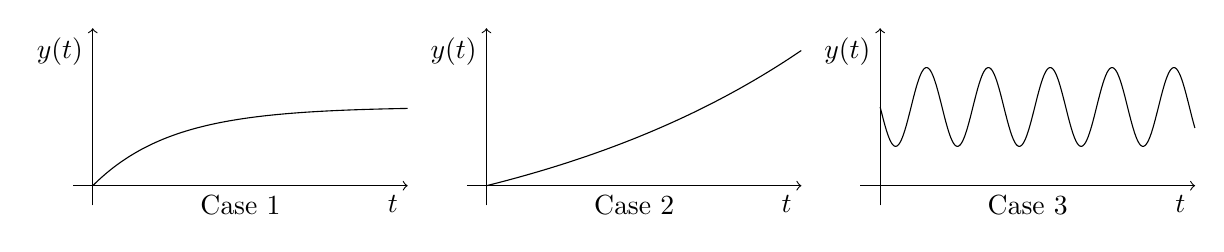
\begin{tikzpicture}
	
	\begin{scope}
	\draw[->] (-0.25,0) -- node[below] {Case 1} (4,0) node[below left] {$ t $};  % x Axis
	\draw[->] (0,-0.25) -- (0,2) node[below left] {$ y(t) $};  % y Axis
	\draw[domain=0:4,samples=500] plot (\x,{1-exp(-\x)});
	\end{scope}
	
	\begin{scope}[shift={(5cm,0cm)}]
	\draw[->] (-0.25,0) -- node[below] {Case 2} (4,0) node[below left] {$ t $};  % x Axis
	\draw[->] (0,-0.25) -- (0,2) node[below left] {$ y(t) $};  % y Axis
	\draw[domain=0:4,samples=500] plot (\x,{exp(0.25*\x)-1});
	\end{scope}
	
	\begin{scope}[shift={(10cm,0cm)}]
	\draw[->] (-0.25,0) -- node[below] {Case 3} (4,0) node[below left] {$ t $};  % x Axis
	\draw[->] (0,-0.25) -- (0,2) node[below left] {$ y(t) $};  % y Axis
	\draw[domain=0:4,samples=500] plot (\x,{1-0.5*sin((180/pi)*8*\x)});
	\end{scope}
	\end{tikzpicture}
\end{center}
Is it possible to look at the expression of $ Y(s) $ and tell which of these situations we have?

\textbf{Yes!}

A final value exists if and only if all poles of $ Y(s) $ are strictly in the LHP, except for a single pole at the origin. 
\begin{itemize}
	\item If $ Y(s) $ has any poles in the RHP, $ y(t) $ is unbounded.
	\item If $ Y(s) $  has a pair of complex conjugate poles on the imaginary axis, the final values is undefined.
\end{itemize}
If a final value exists, it can be found using the \textbf{final value theorem}.  If $ \LT[y]=Y $ and poles of $sY $ lie strictly in the LHP, then the Final Value Theorem states
	\[ 	\lim\limits_{t\to\infty}y(t) = \lim\limits_{s\to0}sY(s) \]
\begin{proof}
	\begin{align*}
	\LT\left[\frac{dy}{dt}\right] &= sY-y(0^-)\\
	sY &=y(0^-) + \LT\left[\frac{dy}{dt}\right]\\
	&=y(0^-)+\int_{0^-}^{\infty}e^{-st}\frac{dy}{dt}(t)dt\\
	\lim\limits_{s\to0}sY(s)&= y(0^-) +\int_{0^-}^{\infty}\frac{dy}{dt}(t)dt\\
	&=y(0^-) + \lim_{t\to\infty}y(t) - y(0^-)\\
	&=\lim_{t\to\infty}y(t) && \qedhere
	\end{align*}
\end{proof}

\exmp
Consider
\[ G(s) = \frac{3}{(s+4)(s+3)} \]
What is the final value for a unit step, $ U(s)=1/s $?
\[ Y(s) = G(s)U(s)=\frac{3}{s(s+4)(s+3)} \]
\[ 	\lim_{t\to\infty}y(t)= \lim\limits_{s\to0}sY(s)= \lim\limits_{s\to0} \frac{3}{(s+4)(s+3)} \]
\[ \lim_{t\to\infty}y(t) = \frac{1}{4} \]
Now consider
\[ G(s) = \frac{3}{(s-4)(s+3)} \]
What is the final value for a unit step, $ U(s)=1/s $? We must be careful! If we apply the FVT blindly, we get 
\[ 	\lim_{t\to\infty}y(t)= \lim\limits_{s\to0}sY(s)= \lim\limits_{s\to0} \frac{3}{(s-4)(s+3)} \]
\[ \lim_{t\to\infty}y(t) = -\frac{1}{4} \]
But, $ y(t) $ is unbounded because there is a pole in the RHP! So, the FVT is only usable if all the poles of $ Y(s) $ are \textbf{strictly} in the LHP (except for a simple pole at the origin). Consider another case where
\[ G(s) = \frac{3}{(s^2+4)} \]
What is the final value for a unit step, $ U(s)=1/s $? The FVT would say that:
\[ 	\lim_{t\to\infty}y(t)= \lim\limits_{s\to0}sY(s)= \lim\limits_{s\to0} \frac{3}{(s^2+4)} \]
\[ \lim_{t\to\infty}y(t) = \frac{3}{4} \]
but again, this would be incorrect because of the poles on the imaginary axis. $ y(t) $ has no final value.

\paragraph*{Initial Value} The initial value $ y(0^+) $ is the value of the response $ y(t) $ at the instance the control input is applied. In a similar manner to the FVT, we can find the initial value $ y(0^+) $. The \textbf{initial value theorem} states that
\[ 	\lim\limits_{s\to\infty}sY(s) \triangleq y(0^+) \]
\begin{proof}
	\begin{align*}
	\LT\left[\frac{dy}{dt}\right] &= sY-y(0^-)\\
	sY &=y(0^-) + \int_{0^-}^{\infty}e^{-st}\frac{dy}{dt}(t)dt\\
	&=y(0^-) + \int_{0^-}^{0^+} \underbrace{e^{-st}}_{=e^{-0t}=1} \frac{dy}{dt}(t)dt + \int_{0^+}^{\infty} e^{-st} \frac{dy}{dt}(t)dt\\
	&=\cancel{y(0^-)} + \big(y(0^+) - \cancel{y(0^-)}\big)+ \int_{0^+}^{\infty}e^{-st}\frac{dy}{dt}(t)dt\\
	&\qquad \text{Now, take the limit of both sides.}\\
	\lim\limits_{s\to\infty}sY(s)&= y(0^+) + \int_{0^-}^{\infty}0\cdot\frac{dy}{dt}(t)dt\\
	&=y(0^+) + 0\\
	\lim\limits_{s\to\infty}sY(s)&=y(0^+)
	\end{align*}
\end{proof}

\exmp
\[ Y(s) = \frac{3}{s(s^2+4)} \]
\[ y(0^+) = \lim_{s\to\infty} sY(s) = \lim_{s\to\infty} \frac{3}{s^2+4} = 0 \]

\paragraph*{Static Gain} The \textbf{static gain} tells you how well a system responds to a step command in the steady-state. The static gain is defined for a step input with magnitude $ a $. Then,
\[ \text{Static Gain}\triangleq \frac{\lim_{t\to\infty}y(t)}{a} \]
Let's look at this using the FVT.
\[ Y(s) = G(s)U(s) \]
So,
\[ \lim_{t\to\infty}y(t) = \lim_{s\to0} sY(s) = \lim_{s\to0} [sG(s)U(s)] \] 
Recall that $ U(s)=a/s $. So,
\[ \lim_{t\to\infty}y(t) = \lim_{s\to0} \left[\cancel{s}G(s)\frac{a}{\cancel{s}}\right] = \lim_{s\to0}[aG(s)] = a G(0) \]
Therefore
\[ \text{Static Gain} = G(0) \]
This is also called the DC Gain in some texts. So, take a system's transfer function and set $ s=0 $ --- that is the system's static gain. Note that this concept only applies if all the poles of $ G(s) $ are strictly in the LHP.

Another way to define static gain: It is the value of $ y(t) $ at steady-state when $ u(t)=1(t) $. This will be equal to $ G(0) $.

\exmp
\[ G(s) = \frac{10(s+7)}{(s+10)(s+20)},\quad u(t)=1(t) \]
Find the initial value, final value, and initial slope of $ y(t) $.
\[ Y(s) = \frac{1}{s}\cdot\frac{10(s+7)}{(s+10)(s+20)} \]
Initial value:
\[ y(0^+) = \lim_{s\to\infty}  sY(s) = \lim_{s\to\infty} \left[ \frac{10(s+7)}{(s+10)(s+20)} \right] \]
\[ y(0^+) = \frac{10\left(\frac{1}{s}+\frac{7}{s^2}\right)}{\left(1+\frac{10}{s}\right)\left(1+\frac{20}{s}\right)} = 0 \]
Final value: First, we can tell the final value exists because all the poles of $ Y(s) $ are strictly in the LHP with just one at the origin. Hence, we can use the FVT.
\[ \lim_{t\to\infty}y(t) = \lim_{s\to0} sY(s) = \lim_{s\to0} \frac{10(s+7)}{(s+10)(s+20)} \]
\[ \lim_{t\to\infty}y(t) = \frac{10(7)}{(10)(20)} = \frac{7}{20} \]
Given that this is a step input, this also means that the Static Gain$ = \frac{7}{20} $.\\
Initial slope: In other words, find $ \dot{y}(0^+) $ (initial value of the derivative of $ y(t) $).
\[ \LT[y(t)] = Y(s) = \frac{10(s+7)}{s(s+10)(s+20)} \]
\[ \LT[\dot{y}(t)] = sY(s) = \frac{10(s+7)}{(s+10)(s+20)} \]
Then, apply the IVT:
\[ \dot{y}(0^+) = \lim_{s\to\infty} (s[sY(s)]) = \lim_{s\to\infty} \frac{10s(s+7)}{(s+10)(s+20)} \]
\[ \dot{y}(0^+) = \frac{10\left(1+\frac{7}{s}\right)}{\left(1+\frac{10}{s}\right)\left(1+\frac{20}{s}\right)} = \frac{10}{1\cdot1} = 10 \]
Sketch of $ u(t) $ and $ y(t) $:
\begin{center}
	\begin{tikzpicture}
	\begin{scope}[shift={(-5cm,0cm)}]
	\draw[->] (-0.25,0) -- (4,0) node[below left] {$ t $};  % x Axis
	\draw[->] (0,-0.25) -- (0,3) node[below left] {$ u(t) $};  % y Axis
	\draw (0,2) node[left] {1} -- (4,2);
	\end{scope}
	\draw[->] (-0.25,0) -- (4,0) node[below left] {$ t $};  % x Axis
	\draw[->] (0,-0.25) -- (0,3) node[below left] {$ y(t) $};  % y Axis
	\draw[domain=0:4,samples=500] plot (\x,{(20/7)*(7/20 - (13/20)*exp(-20*(\x/8)) + (3/10)*exp(-10*(\x/8)))});
	\draw[dashed] (0,0) -- ++(1.5/8,1.5*7/20) -- ++(1.5/8,1.5*7/20) -- ++(1.5/8,1.5*7/20) node[right] {$ m=10 $};
	\draw[dashed] (0,1) node[left] {$ \frac{7}{20} $}-- (4,1);
	\end{tikzpicture}
\end{center}

\exmp
\[ G(s) = \frac{s-2}{(s+1)(s+4)} \]
Sketch the output to a unit ramp input.
\[ U(s) = \frac{1}{s^2} \quad\Rightarrow\quad Y(s) = \frac{s-2}{s^2(s+1)(s+4)} \]
$ Y(s) $ has two poles at the origin --- therefore, there is no final value! Let's look at the initial value and initial slope:
Initial value:
\[ y(0^+) = \lim_{s\to\infty} sY(s) = \lim_{s\to\infty} \left[ \frac{s-2}{s(s+1)(s+4)} \right] = 0 \]
Initial slope:
\[ \LT[y(t)] = Y(s) = \frac{s-2}{s^2(s+1)(s+4)} \]
\[ \LT[\dot{y}(t)] = sY(s) = \frac{s-2}{s(s+1)(s+4)} \]
Then, apply the IVT:
\[ \dot{y}(0^+) = \lim_{s\to\infty} (s[sY(s)]) = \lim_{s\to\infty} \frac{s-2}{(s+1)(s+4)} = 0 \]
So, we have an initial value and initial slope of zero, and we cannot obtain a final value. Note, however, that slope transfer function
\[ \LT[\dot{y}(t)] = \frac{s-2}{s(s+1)(s+4)} \]
admits a final value. So, we can find a final slope.
\[ \lim_{t\to\infty}\dot{y}(t) = \lim_{s\to0}s^2Y(s) = \lim_{s\to0} \frac{s-2}{(s+1)(s+4)} = \frac{-2}{4} = -\frac{1}{2}\]
Although we will not go over the steps here, it can be found that
\[ y(t) = \left(\frac{7}{8} - e^{-t} + \frac{1}{8}e^{-4t} -\frac{1}{2}t\right)1(t) \]
This confirms our finding:
\begin{itemize}
	\item Initial value $ y(0^+)=\frac{7}{8} - 1 + \frac{1}{8} - 0 = 0 $
	\item Initial slope $ \dot{y}(0^+)=0 + 1 - \frac{4}{8} - \frac{1}{2} = 0 $
	\item No final value (as the $ -\frac{1}{2}t $ term will continue growing)
	\item Final slope $ \lim\limits_{t\to\infty} \dot{y}(t) = 0 - 0 + 0 -\frac{1}{2} = -\frac{1}{2} $
\end{itemize}
Additionally, we can see that as $ t $ becomes large, $ y(t)\approx \dfrac{7}{8} - \dfrac{1}{2}t $. 
\begin{center}
%	\begin{tikzpicture}
%	\draw[->] (-0.5,0) -- (6,0) node[below left] {$ t $};  % x Axis
%	\draw[->] (0,-3) -- (0,3) node[below left] {$ y(t) $};  % y Axis
%	\draw[domain=0:6,samples=500] plot (\x,{7/8 - exp(-\x) + (1/8)*exp(-4*\x) - 0.5*\x});
%	\draw[dashed] (0,0) -- (3,3) node[right] {$ u(t) $};
%	\draw[dashed] (7/4,0) -- node[right] {\footnotesize Steady State Asymptote} (6,-2.125);
%	\draw[dotted] (0,0) -- node[below left,align=right] {\footnotesize Steady State slope}(6,-3);
%	\end{tikzpicture}
	\begin{tikzpicture}[scale=1.5]
	\draw[->] (-0.5,0) -- (4,0) node[below left] {$ t $};  % x Axis
	\draw[->] (0,-2) -- (0,2) node[below left] {$ y(t) $};  % y Axis
	\draw[domain=0:4,samples=500] plot (\x,{7/8 - exp(-\x) + (1/8)*exp(-4*\x) - 0.5*\x});
	\draw[dashed] (0,0) -- (2,2) node[right] {$ u(t) $};
	\draw[dashed] (7/4,0) -- node[right] {\footnotesize Steady State Asymptote} (4,-1.125);
	%\draw[dotted] (0,0) -- node[below left,align=right] {\footnotesize Steady State slope}(4,-2);
	\draw[dotted] (0,7/8) node[left] {$ y=\frac{7}{8} $}  -- (7/4,0) node[above right] {$ t=\frac{7}{4} $};
	\node at (1.25,0.5) {slope$ =-1/2 $}; % improve this
	\end{tikzpicture}
\end{center}

\exmp
\[ G(s) = \frac{20}{s^2+6s+144} \]
What is the Static Gain? (The final value of output for input $ 1(t) $.) First, what are the poles of $ G(s) $?
\[ s^2+6s+144 \quad\Rightarrow\quad s = -3 \pm \frac{\sqrt{36-4\cdot144}}{2} = -3\pm j\sqrt{135}  \]
So, the static gain exists. Then,
\[ \text{Static Gain} = G(0) = \frac{20}{144} \approx 0.14 \]

\end{document}

